\documentclass[CS5104-Notes.tex]{subfiles}
\begin{document}

\section{Neural networks}

\subsubsection{Issue with logistic regression}
In logistic regression, when there are many input features in combination with a complex non-linear hypothesis, the number of features used grows very dramatically. For example in a small image of $50\times50$ pixels, there are 2500 features, which leads to over 3 million features with a quadratic model. This is computationally too expensive, making it difficult to choose a good polynomial.
\n
Therefore, a different, more effective method was explored, which led to neural networks.

\subsection{Neural network}
A neural network is a biologically inspired method which tries to copy the way the brain works for classification and prediction. This method has recently become popular because of the increase in computation power with GPUs allow for the ability to deal with large scale networks and large datasets. Previously neural networks were not very effective as they were too small and worked on small datasets.

\subsubsection{Artificial neuron}
An artificial neuron is modelled like a neuron in the human brain. It takes a series of inputs and outputs a single value. The weights that modifier the input values act as the $\theta$ parameters that have to be adjusted during training. 
\begin{figure}[H]
  \centering
  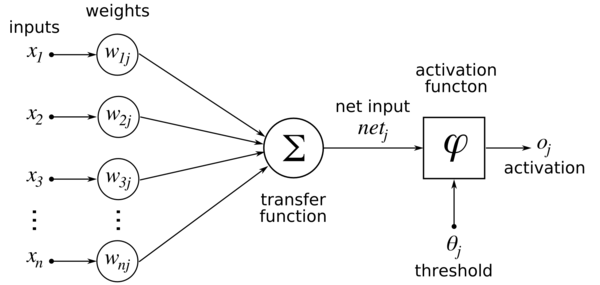
\includegraphics[width=0.75\textwidth, keepaspectratio]{imgs/artificial-neuron.png}
  \caption{A single artificial neuron.}
\end{figure}
\noindent
In addition to the inputs $x_{1}, x_{2}, ..., x_{n}$ a bias unit $x_{0}$ is often added that helps shift the activation function left or right. For the activation function, a sigmoid (logistic) activation function is often used
\begin{equation}
h_{\theta}(x) = g(\theta^{T}x) = \frac{1}{1 + e^{-\theta^{T}x}}
\end{equation}
A neural network is made up for a network of artificial neurons, most notably the input, hidden layers and output layer.

\subsubsection{Artificial network}
The combination of many neurons and layers creates a neural network. The network's layer are connected by passing the output of one layer in as the inputs to the next layer. In most cases, all output from one layer is used for the next layer and the weight help balance which inputs are more important for each particular neuron.
\begin{figure}[H]
  \centering
  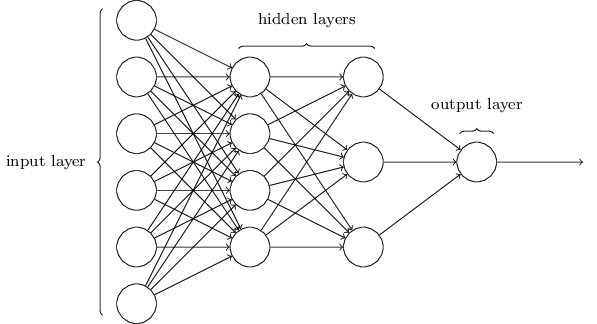
\includegraphics[width=0.7\textwidth, keepaspectratio]{imgs/artificial-network.png}
  \caption{Example of an artificial network with 2 hidden layers.}
\end{figure}
\noindent
At each step of the computation, the activation function of the next layer is the sum of the inputs and weights ($w$ or $\theta$), for example
\begin{equation}
a_{1}^{(2)} = g(\theta_{10}^{(1)}x_{0} + \theta_{11}^{(1)}x_{1} + \theta_{12}^{(1)}x_{2})
\end{equation}
for the first neuron in the second layer. $\theta_{j}^{(i)}$ specifies the weight parameter for the $j$th neuron of the $i$th layer. For a single two-class classification, only one output neuron is needed where the output 0 specifies the data is not of the class and output 1 specifies the data is of the class.

\subsubsection{Multiclass classification}
In multiclass classification, it is not as easy as using a range to specify the different classes (like 0-0.3, 0.3-0.6, 0.6-0.9). Rather we will want to use a vector to specify each class, for example
\n
\begin{minipage}{0.31\textwidth}
  $h_{\theta}(x) \approx \begin{bmatrix} 1 \\ 0 \\ 0 \end{bmatrix}$ for class 1
\end{minipage}
\begin{minipage}{0.31\textwidth}
$h_{\theta}(x) \approx \begin{bmatrix} 0 \\ 1 \\ 0 \end{bmatrix}$ for class 2
\end{minipage}
\begin{minipage}{0.31\textwidth}
$h_{\theta}(x) \approx \begin{bmatrix} 0 \\ 0 \\ 1 \end{bmatrix}$ for class 3
\end{minipage}


\subsubsection{Backpropagation algorithm}
Backpropagation in neural networks is a method of minimising the cost function by finding the best $\theta$ values. The initial computation from training passes through the network via forward propagation to return an output value. To adjust the weights on the next training iteration, the error between the predicted output and actual output must be propgated backwards through the network.
\n
For example, in a four layer network, the result $a_{j}^{(4)}$ is the output at the output layer. The error for the result is defined as
\begin{equation}
\delta_{j}^{(4)} = a_{j}^{(4)} - y_{j}
\end{equation}
where $y_{j}$ is the actual output. This can be written as
\begin{equation}
\delta^{(4)} = a^{(4)} - y
\end{equation}
to express everything in vector form. This is the error of the output layer. The error for all previous layers is then defined as
\begin{equation}
\delta^{(l)} = (\theta)^{T}\delta^{(l+1)} \times g'(z^{(l)})
\end{equation}
where $g'(z^{(l)})$ is the derivative of the activation function $g()$ evaluted at the input values $z^{(l)}$ Note the error $\delta^{(l+1)}$ is used to define the error of the current layer. Furthermore, the multiplication used $\times$ is an element wise multiplication of the vectors.

\begin{algorithm}[H]
\begin{algorithmic}[1]
\Procedure{Backpropagation}{}
\For{$m$ training samples}
  \State Set $\Delta_{ij}^{(l)} = 0$ for all $l,i,j$
  \For{$i = 1$ to $m$}
    \State Set $a^{(1)} = x^{(i)}$
    \State \textsc{ForwardPropagation} to compute $a^{(l)}$ for $l = 2,3,...,L$
    \State $\delta^{(L)} = a^{(L)} - y^{(i)}$
    \For{$l = L - 1$ to $2$}
      \State $\delta^{(l)} = (\theta^{(l)})^{T}\delta^{(l+1)} \times g'(z^{(l)})$
    \EndFor
    \State $\Delta_{ij}^{(l)} = \Delta_{ij}^{(l)} + a_{j}^{(l)}\delta_{i}^{(l+1)}$
  \EndFor
\EndFor
\EndProcedure
\end{algorithmic}
\caption{Backpropagation algorithm for neural networks.}
\end{algorithm}
The backpropagation algorithm gives a final change
\begin{align}
  D_{ij}^{(l)} &= \frac{1}{m}\Delta_{ij}^{(l)} + \lambda\theta_{ij}^{(l)} \text{ if } j \neq 0 \\
  D_{ij}^{(l)} &= \frac{1}{m}\Delta_{ij}^{(l)} \text{ if } j = 0
\end{align}
$D_{ij}^{(l)}$ is the change to all weights, indexed by $l,i,j$. It is in fact the partial derivative of the cost function $J(\theta)$ with respect to each $\theta$ parameter
\begin{equation}
D_{ij}^{(l)} = \frac{\partial J(\theta)}{\partial \theta_{ij}^{(l)}}
\end{equation}

\subsubsection{Gradient checking}
Because the backpropagation algorithm can be a difficult algorithm to debug, especially with off-by-one errors in the layer index or neuron index. A derivative checking procedure can be used to check the correctness of the backpropagation implementation. This is not done except for debugging purposes in general, because it is very slow to compute.
\begin{figure}[H]
  \centering
  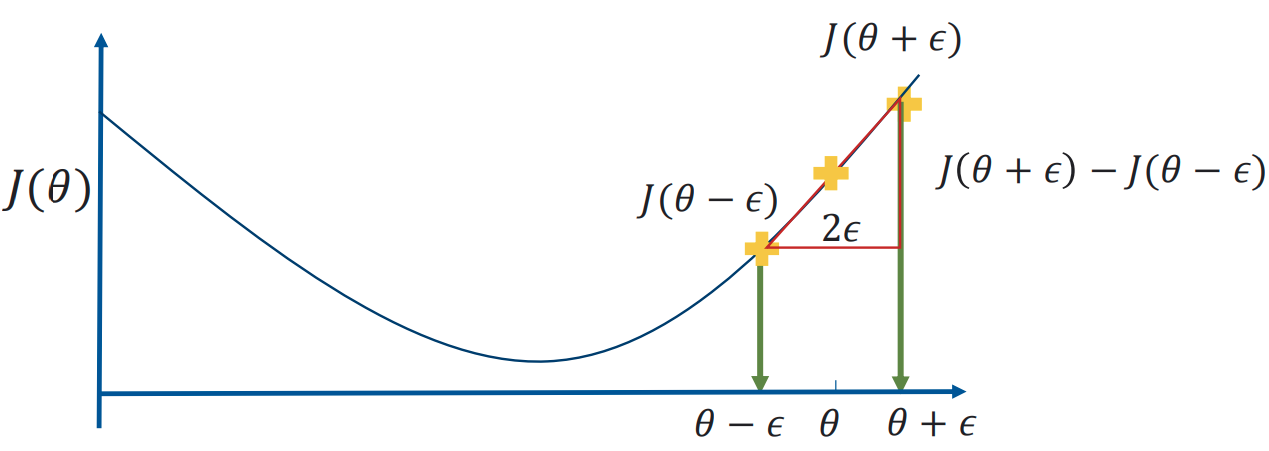
\includegraphics[width=0.9\textwidth, keepaspectratio]{imgs/gradient-checking.png}
\end{figure}
\noindent
At any specific value of $\theta$, the derivative can be numerically estimated as
\begin{equation}
\frac{dJ(\theta)}{d\theta} \approx \frac{J(\theta + \epsilon) - J(\theta - \epsilon)}{2\epsilon}
\end{equation}
In practice, $\epsilon$ is set to a small value such as $10^{-4}$. Gradient checking is used to compare the derivative from backpropagation against the numerical estimate. 

\end{document}